\section{MVP}

Para validar a ideia desta bancada foi proposto um mínimo produto viável (MVP) que possuísse as principais características da solução proposta, mas que pudesse ser construído com materiais já disponíveis pela equipe.

Do ponto de vista de projeto mecânico, esta primeira versão da bancada teve sua estrutura construída em madeira, utilizou corrediças de gaveta para dar liberdade de movimento no eixo X e usava como torre uma estrutura de aço. A escolha por estas soluções se deu pela já disponibilidade das mesmas na equipe Céu Azul.

Do ponto de vista de projeto eletrônico todos os componentes já estavam presentes, com exceção do Pitot de múltiplas tomadas, das células de carga e dos módulos HX711.

Do ponto de vista de software o aplicativo para controle da bancada foi desenvolvido de forma preliminar enquanto o software de tratamento e analise de dados ainda não existia.

As figuras \ref{fig:bancada11}a e \ref{fig:bancada12}b mostram o MVP finalizado.

\begin{figure}[!ht]
    \centering
    \caption{Primeira versão da bancada - MVP. Fonte: Lehmkuhl(2018)}
        \subfloat[]{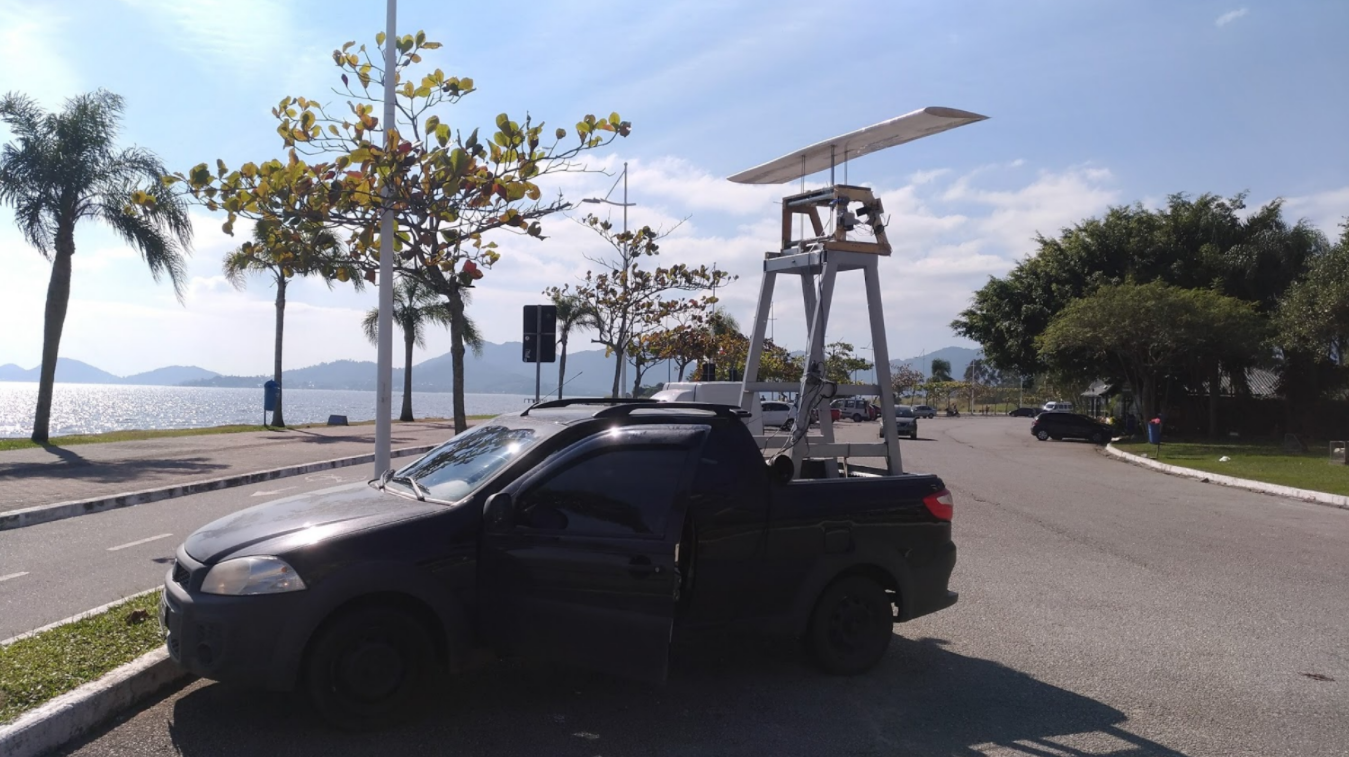
\includegraphics[width=0.4\columnwidth]{figuras/testes/bancada_mvp_1.png}}
        \label{fig:bancada11}
        \qquad
        \subfloat[]{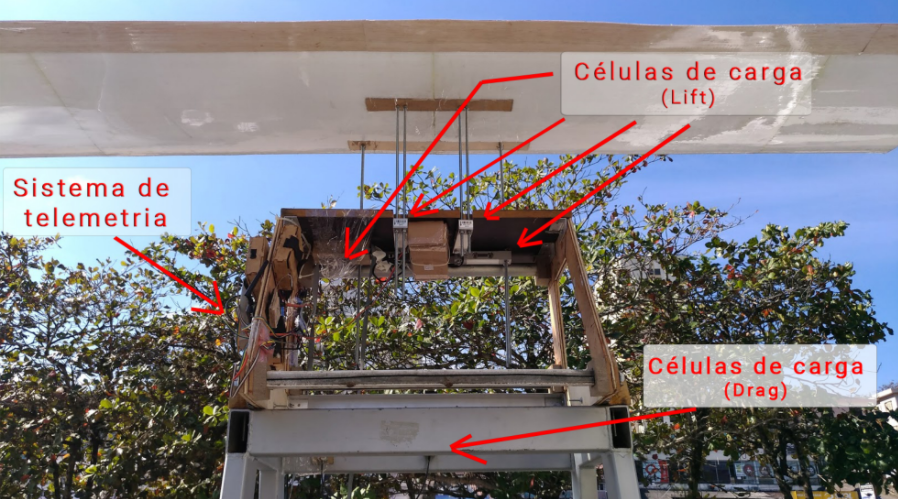
\includegraphics[width=0.4\columnwidth]{figuras/testes/bancada_mvp_2.png}}
        \label{fig:bancada12}
\end{figure}

Foi realizada uma serie de testes com esta bancada, entre eles o de medição de forças aerodinâmicas em uma asa, de medição do empuxo dinâmico em motor e de medição do momento causado pelo acionamento de superfícies de comando (ailerons) em uma asa. O procedimento destes testes e seus resultados esta detalhado em Lehmkuhl (2018). 

O MVP foi um sucesso no sentido de que provou o funcionamento da bancada proposta em curto espaço de tempo, porém possuía problemas estruturais intrínsecos as escolhas para a prototipagem mecânica, não demonstrando repetibilidade suficiente dos resultados. Além disso, ficaram claros diversos problemas do ponto de vista de execução, levantados por Lehmkuhl (2018), entre eles:

\begin{itemize}
    \item Aplicativo ainda em estágio inicial, apresentando uma interface pouco intuitiva
    \item Dificuldade para se ajustar o ângulo de incidência do dispositivo testado
    \item Problemas recorrentes de mal-contato elétrico, resultando na perda de baterias inteiras de dados
    \item Pouco controle sobre o estado e funcionamento do computador da bancada
    \item Configuração do teste no computador da bancada era realizado modificando-se o script original, o que tornava esta configuração bastante suscetível a erros pelo operador 
    \item Software embarcado (no computador da bancada) pouco organizado, com as estruturas de funcionamento do software altamente entrelaçadas, dificultando sua expansão e manutenção
    \item Falta de sincronia entre os dados das células de carga com relação aos outros sensores, o que tornava o processamento dos dados um processo bastante massante
    \item Falta de informações sobre o teste no arquivo de gravação dos dados, o que fazia com que o operador precisasse recorrer a outros meios para guardar a informação sobre o que e como estava sendo feito em cada bateria de testes, causando muitas vezes a perda de informação sobre as mesmas
    \item Falta de software para analise dos dados, o que tornava o processo de utilização dos dados gerados pela bancada uma tarefa altamente especializada
\end{itemize}

Estes pontos foram tomados como base para a segunda versão da bancada, detalhada neste texto e denominada "Bancada V1".

\section{Bancada V1}

Levando em conta os pontos levantados no MVP deu-se inicio a modelagem e construção da Bancada V1.

% \subsection{Modelo físico}

% COMENTAR SOBRE O MODELO ESTATICO E A CORRECAO DE FALSA SUSTENTACAO

\subsection{Mecânica}

A estrutura da bancada utilizando perfis extrudados em alumínio foi modelada no software Solidworks e é mostrada ja na figura \ref{fig:estrutura_bancada} para facilidade de entendimento das partes.

\begin{figure}[!ht]
    \centering
    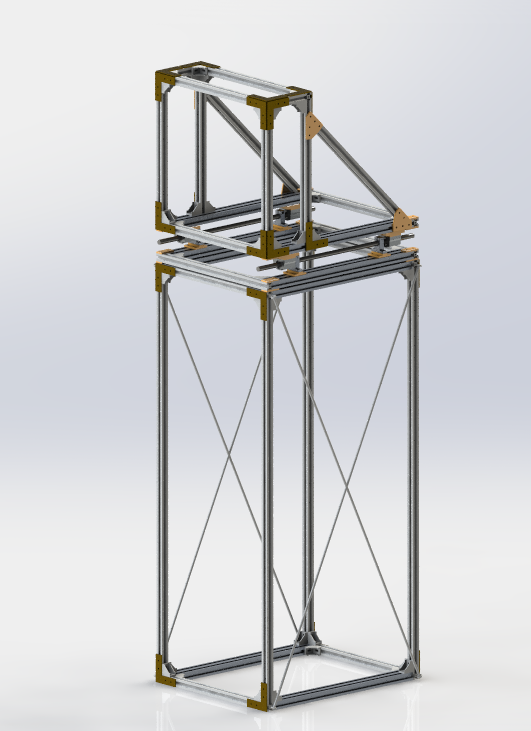
\includegraphics[width=.7\linewidth]{figuras/renders/estrutura_bancada_completa.png}
    \caption{Estrutura da bancada com conexões. Fonte: O autor.}
    \label{fig:estrutura_bancada}
\end{figure}

Os perfis de alumínio são adquiridos em barras de 1 metro de comprimento. A modelagem permitiu assim a definição das medidas dos cortes a serem realizados e a otimização do uso das barras.

% Para o projeto decidiu-se por evitar deslocamentos horizontais e verticais maiores que 1mm. Esta restrição visa limitar a 0.5 graus o ângulo maximo devido a deformaçao da balança em pitch em o acoplamento das mediçoes de sustenta que a deformação da bancada induza erros de alinhamento e consequentemente misture as medidas de sustentação e arrasto \cite{gonzalez2011components}.

As conexões estruturais foram feitas com cantoneiras planas de aço, garantindo rigidez nas juntas, agregando fidelidade na simulação (uma vez que nela as juntas são consideradas rígidas).

Para o encaixe das células de carga na bancada, assim como dos suportes das guias lineares e dos \textit{pillow-blocks}, foram projetados adaptadores que posteriormente foram produzidos via manufatura aditiva de polímero (figura \ref{adaptador_pillow}). Este método de manufatura permitiu a rápida prototipagem dessas peças e acelerou o desenvolvimento do projeto.

\begin{figure}[!ht]
    \centering
    \caption{Adaptadores impressos para as células de carga. Fonte: O autor.}
        \subfloat[Adaptadores para encaixe das células de carga de sustentação e momento.]{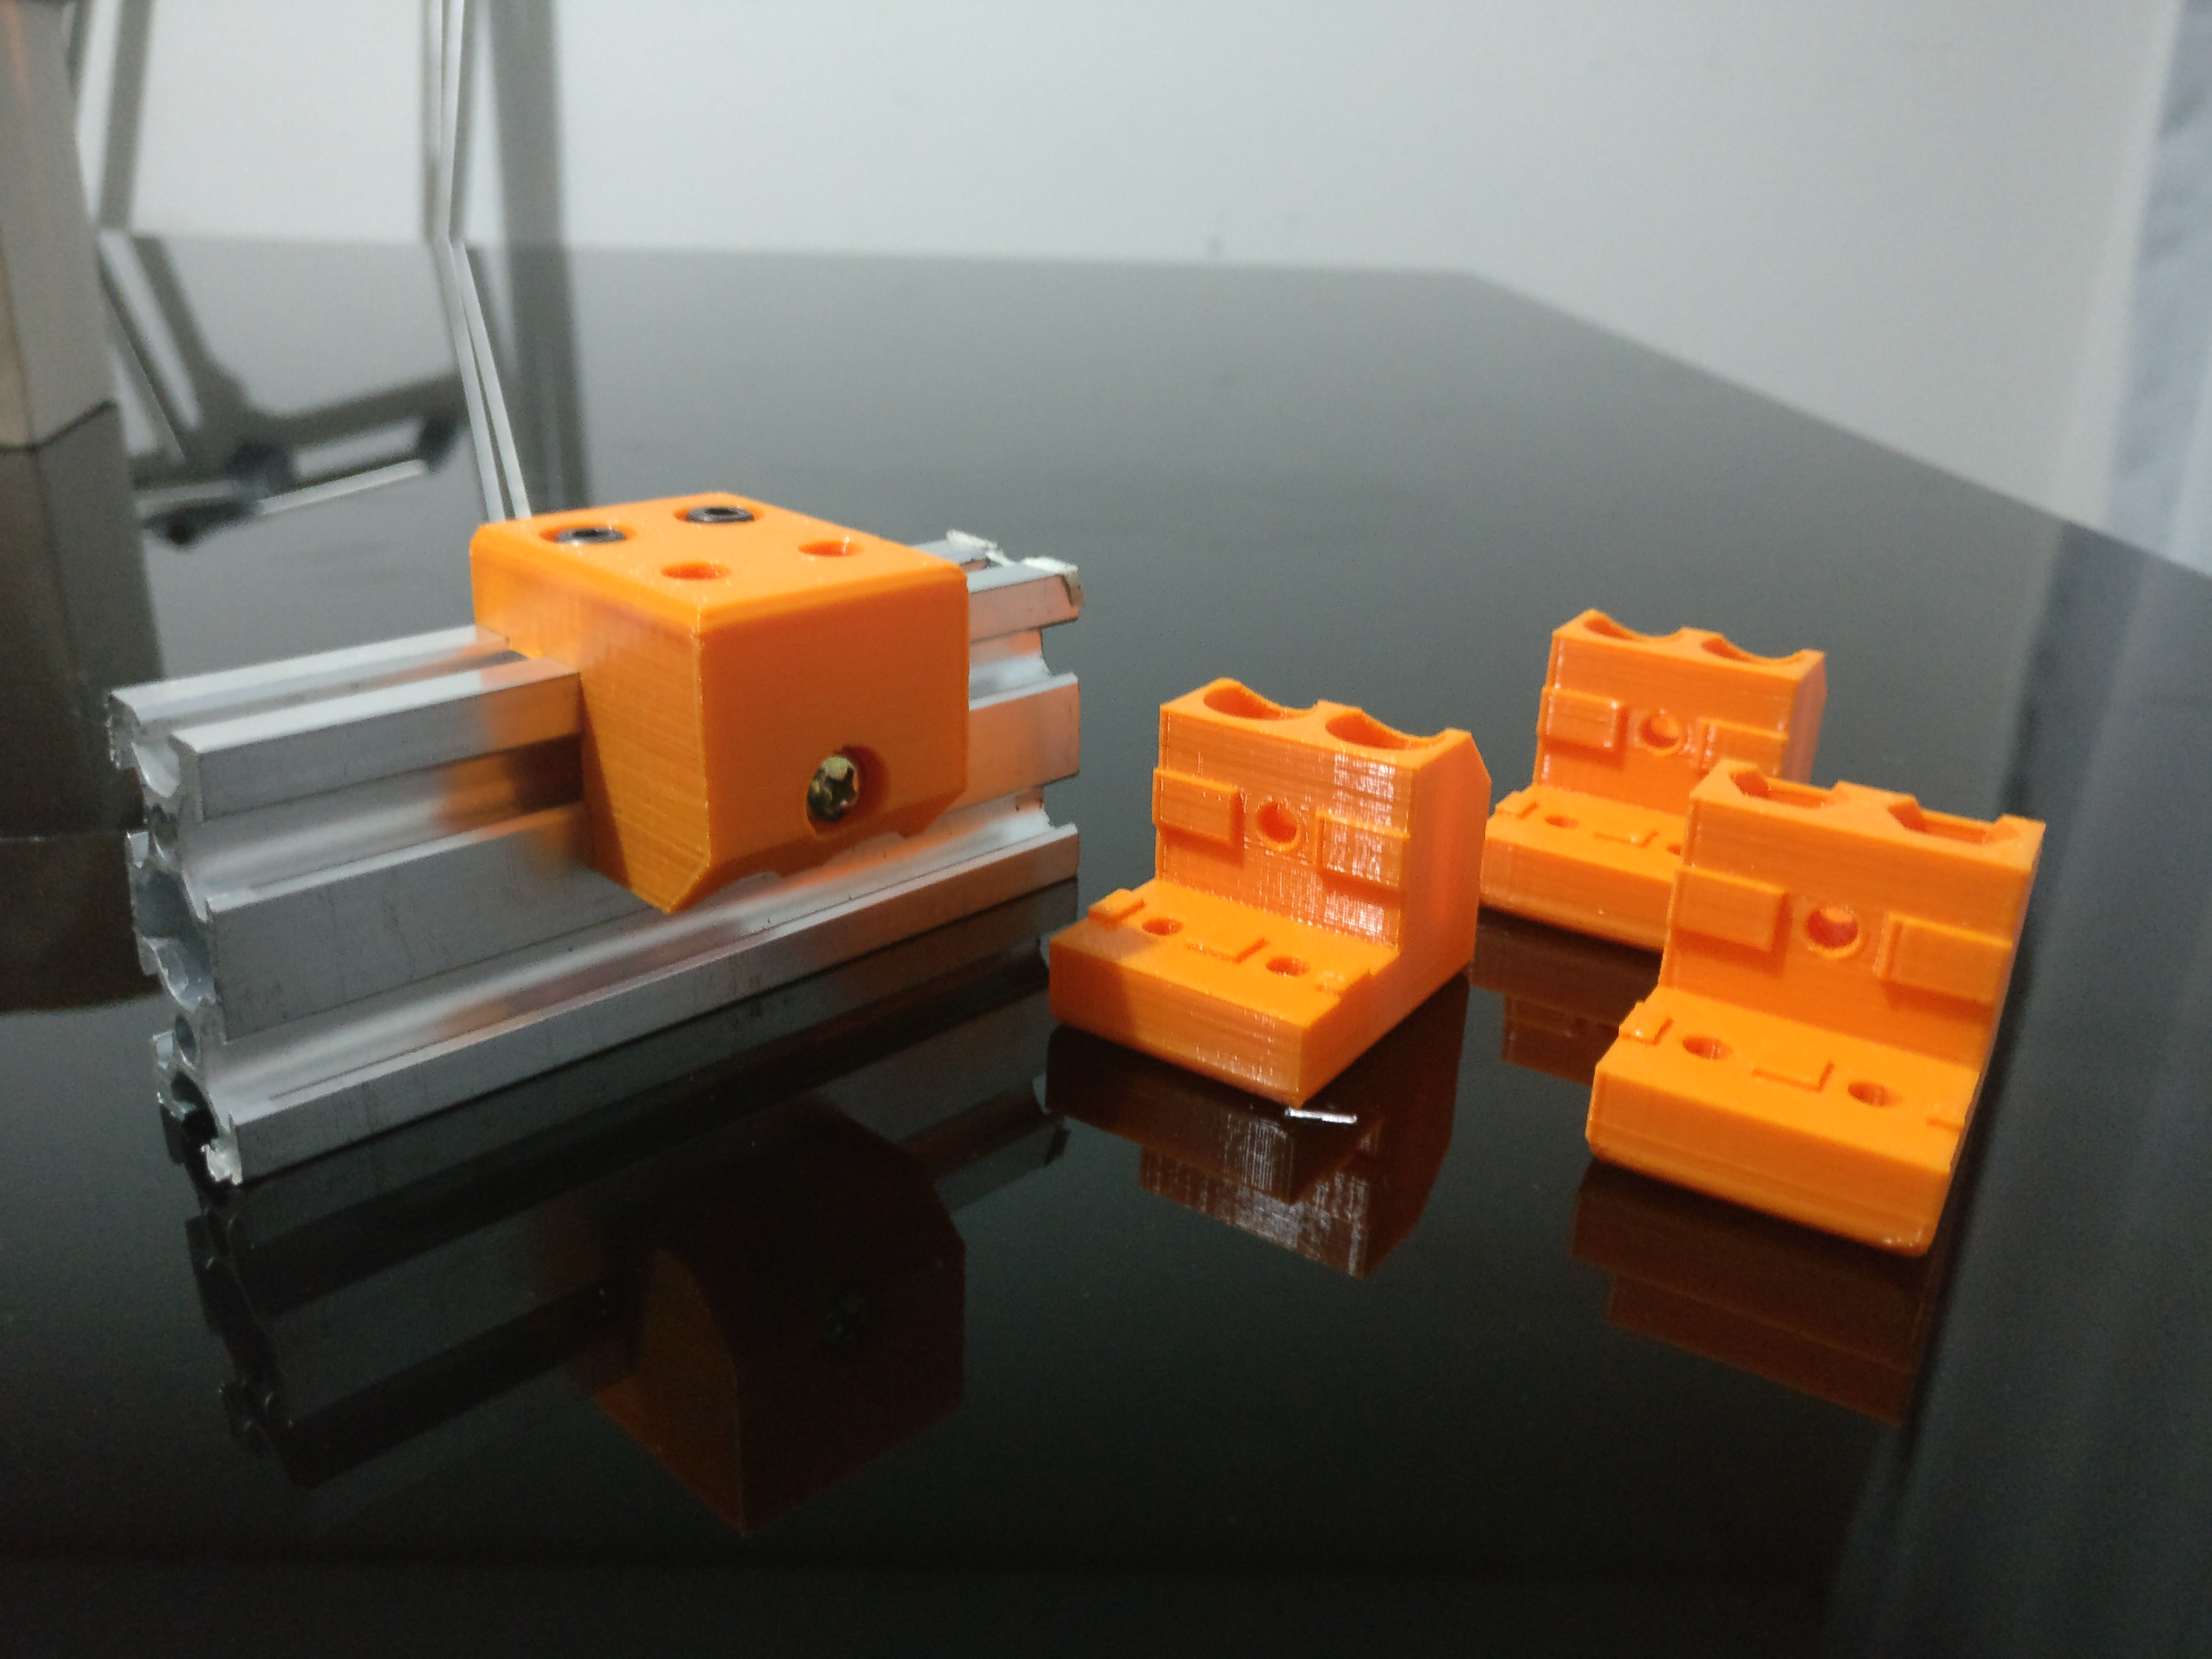
\includegraphics[width=0.4\columnwidth]{figuras/construcao/suporte_reforcado_celulas_3.jpg}}
        \label{encaixe_celulas_sustentacao}
        \qquad
        \subfloat[Células de carga de sustentação e momento com adaptador.]{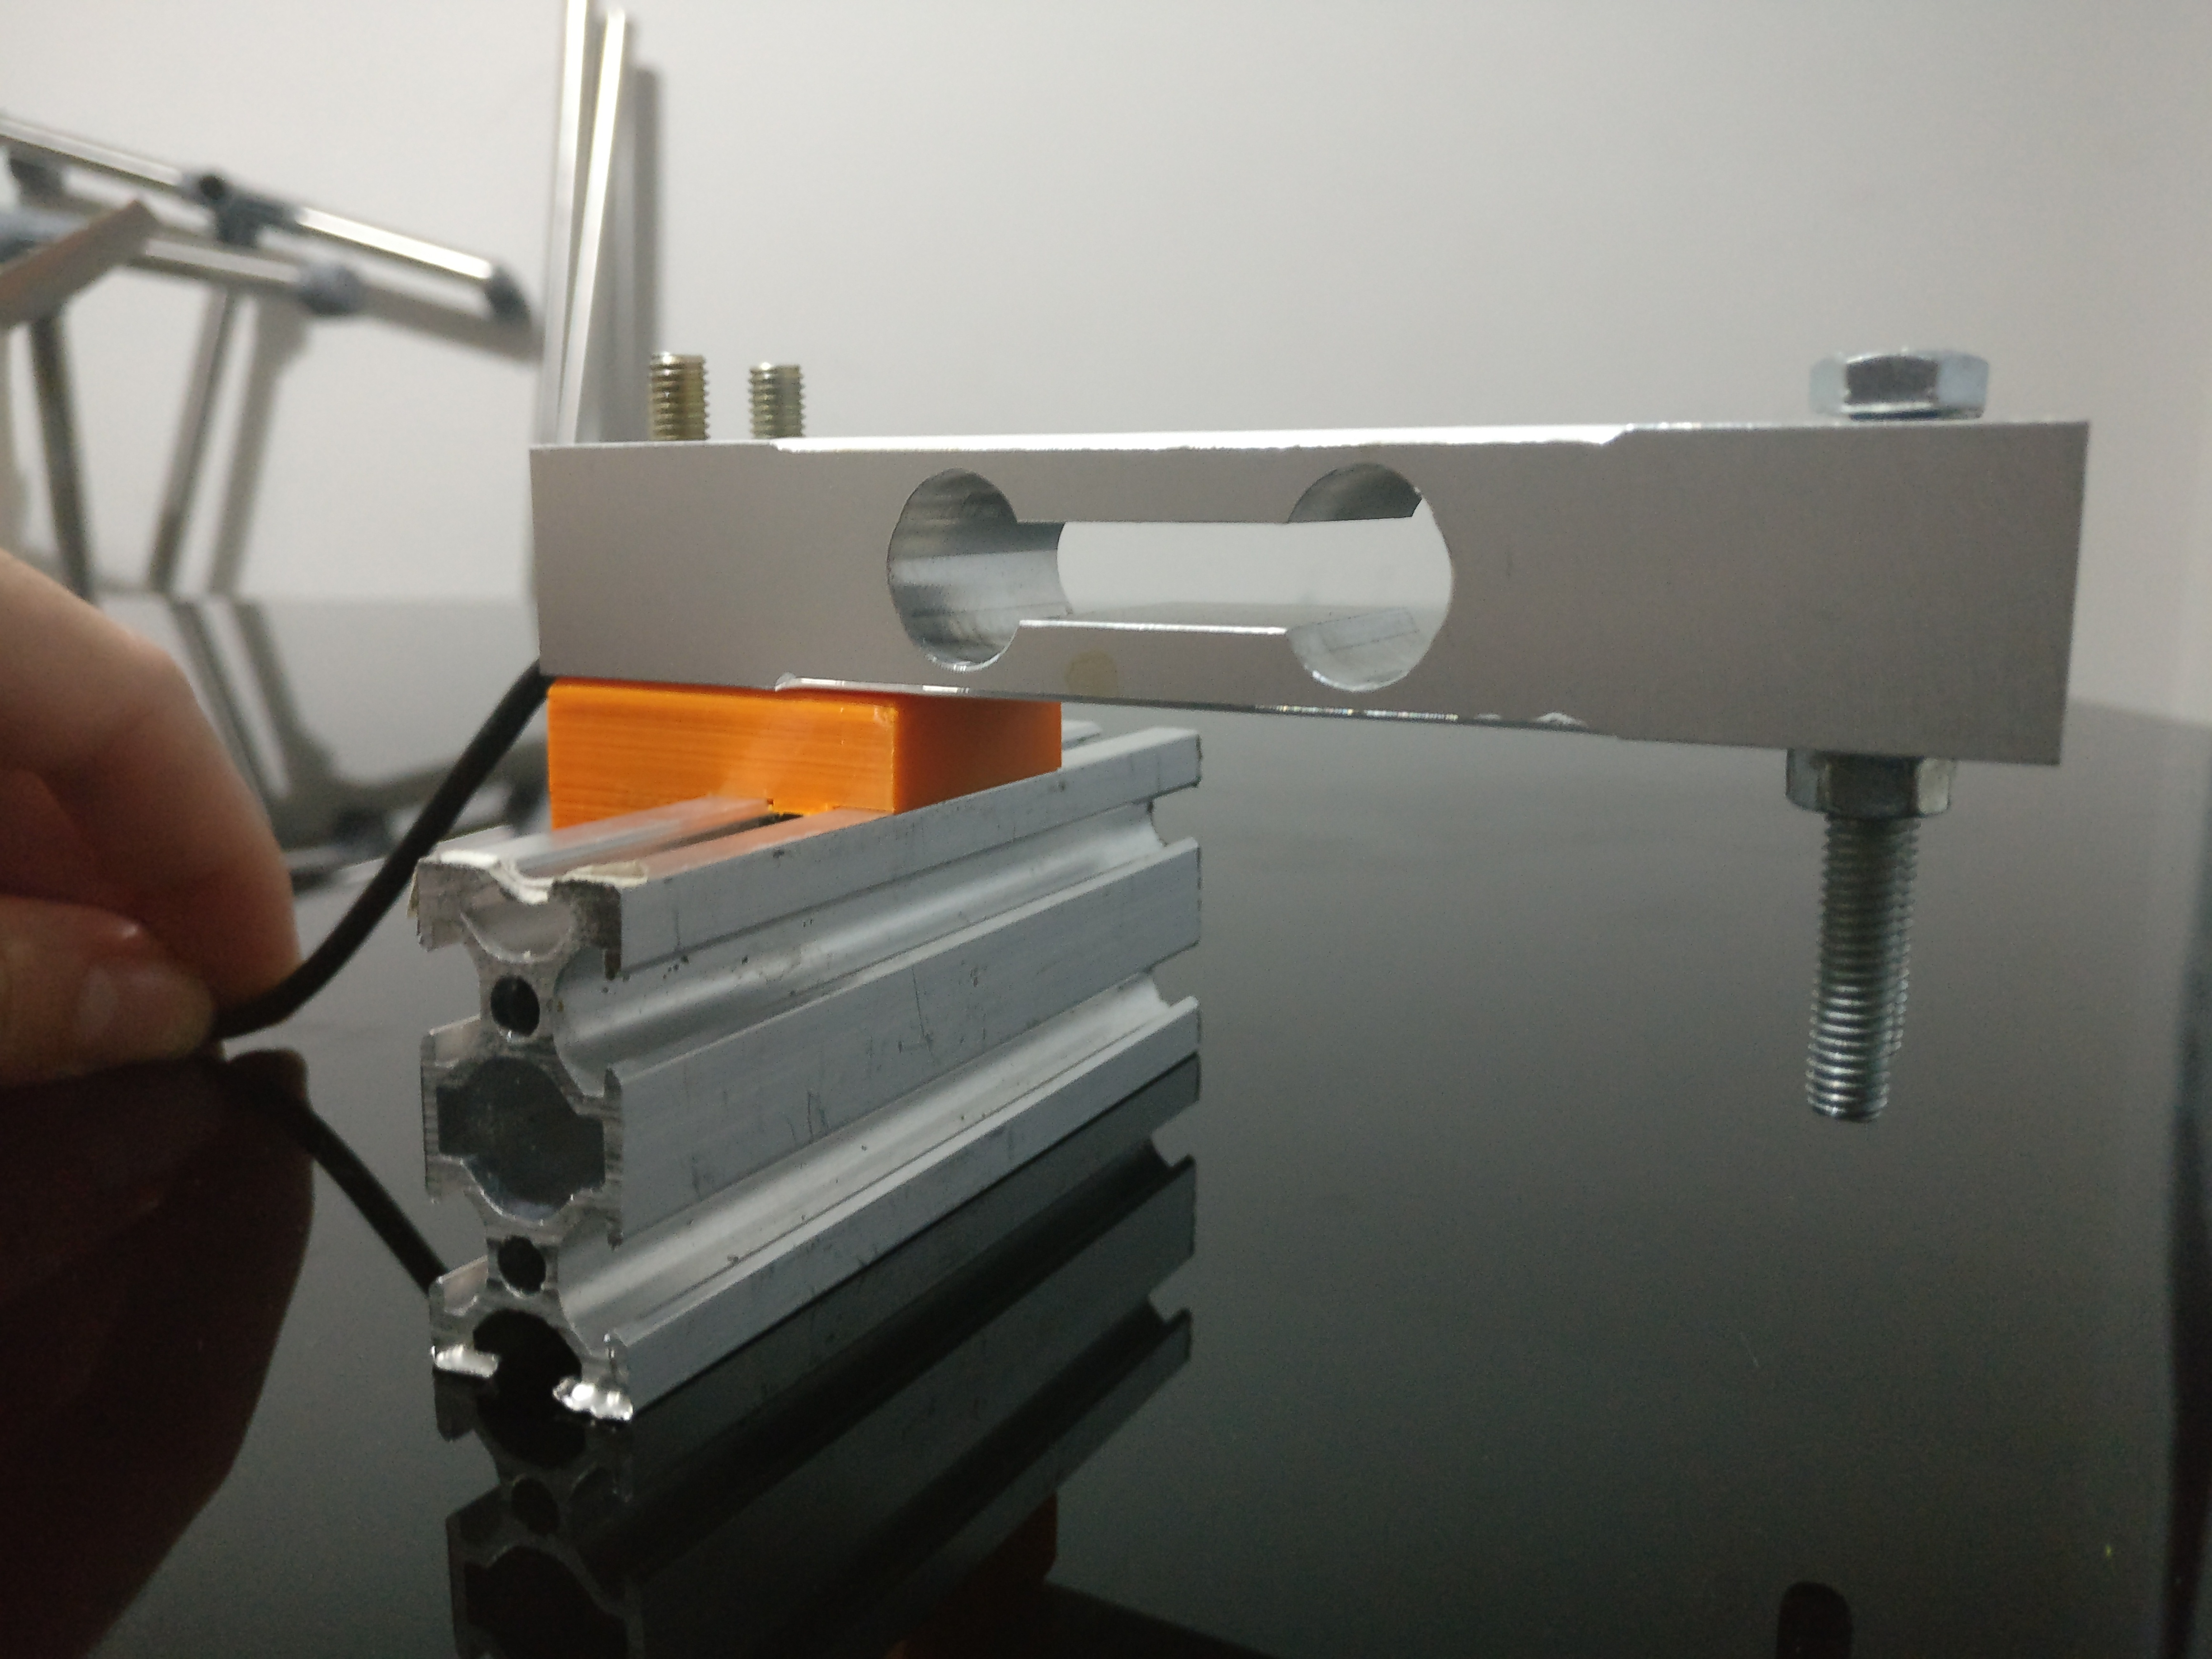
\includegraphics[width=0.4\columnwidth]{figuras/construcao/suporte_reforcado_celulas_1.jpg}}
        \label{encaixe_celulas_sustentacao_2}
\end{figure}

\begin{figure}[!ht]
    \centering
    \caption{Adaptadores para Pillow-Block e Suporte SK12. Fonte: O autor.}
        \subfloat[Adaptador para encaixe do Pillow Block ("carrinho") na bancada.]{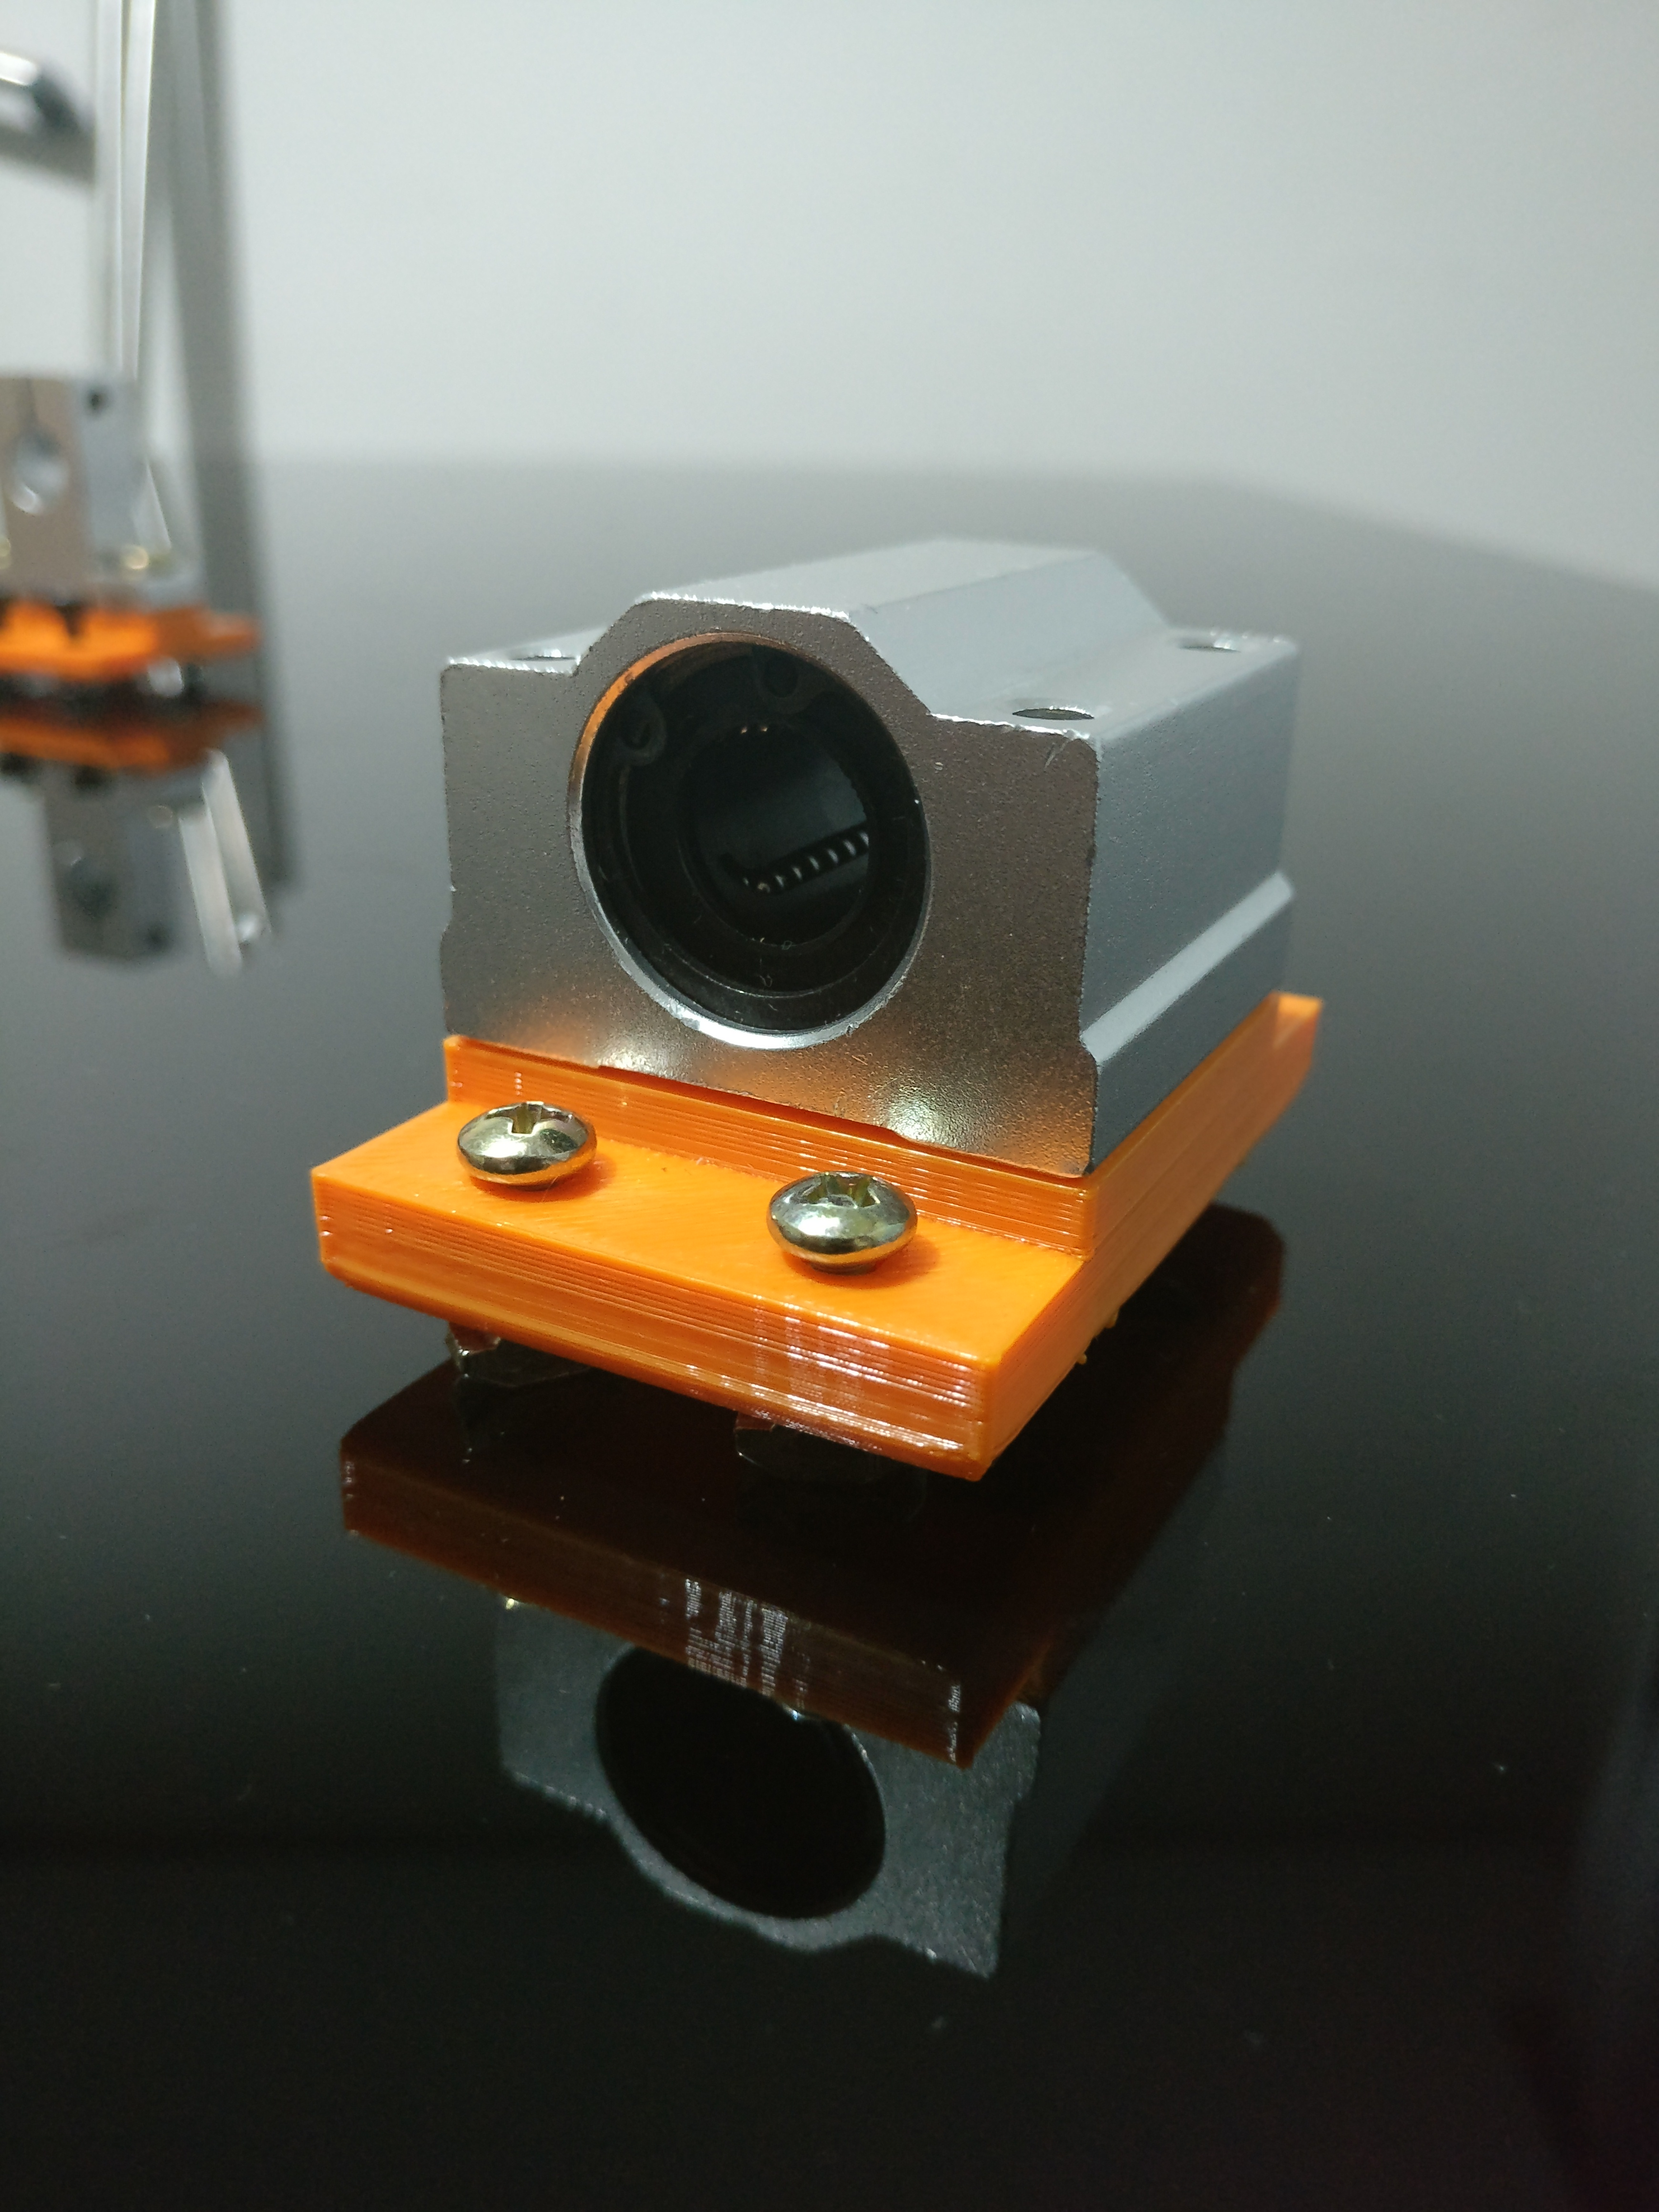
\includegraphics[width=0.4\columnwidth]{figuras/construcao/encaixe_pillow.jpg}}
        \label{adaptador_pillow}
        \qquad
        \subfloat[Adaptador para encaixe dos suportes das guias lineares na bancada.]{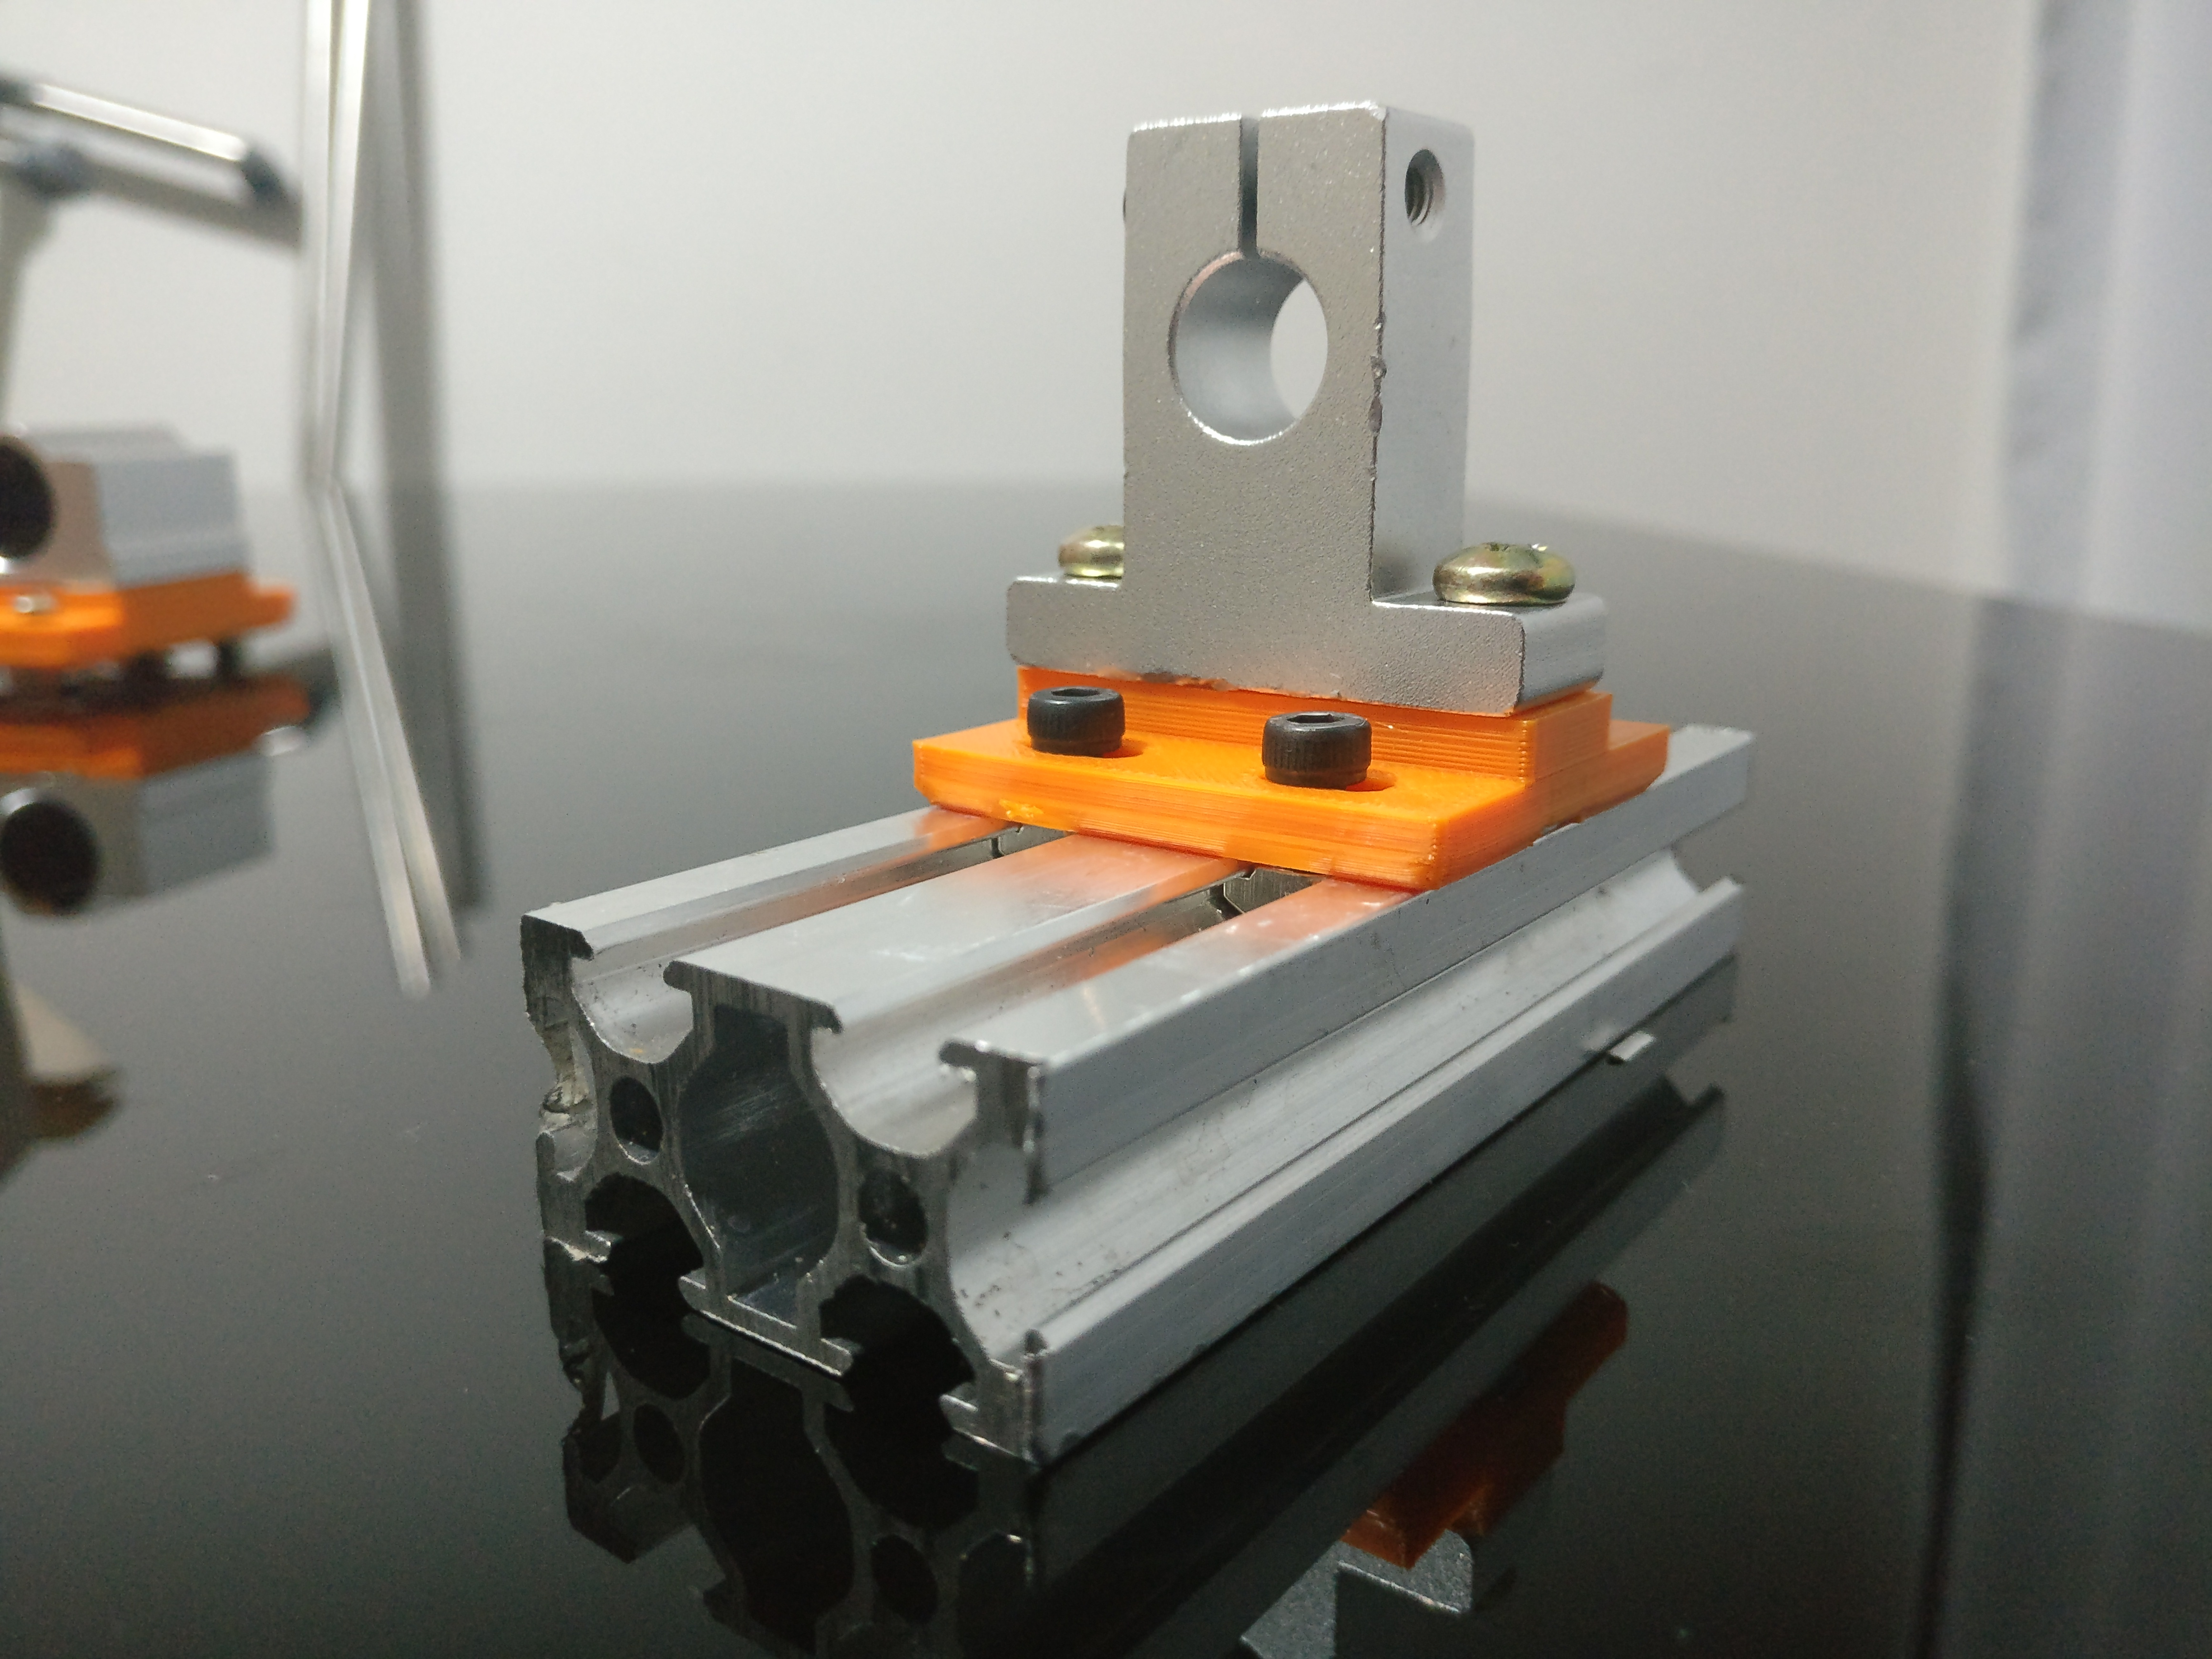
\includegraphics[width=0.4\columnwidth]{figuras/construcao/encaixe_sk12.jpg}}
        \label{adaptador_sk12}
\end{figure}

Devido à dificuldade na simulação de peças produzidas por este processo, que possuem alta anisotropia e grande dispersão nos resultados dependendo da qualidade da impressão \citep{montero2001material}, foram realizados testes estruturais estáticos para se garantir que as peças não falhassem.

Cabe aqui um adendo de que, para se garantir ainda maior rigidez à bancada como um todo, é de interesse a produção dessas peças em metal, realizando as devidas modificações para melhor se adequar ao processo de manufatura escolhido. A produção dessas peças em metal contudo não foi realizada dentro do tempo do presento trabalho.

Dado que a bancada não teve seu movimento em X restrito exclusivamente por células de carga (como foi o caso no eixo Z), foi necessário permitir liberdade de movimento neste sentido, de modo que o carregamento se desse quase que exclusivamente na célula de carga. Para isto foram instaladas guias lineares nesta direção (figura \ref{guias_lineares}). Esta solução possui baixo atrito, além de apresentar pouquíssima folga no sentido transversal ao eixo da guia, o que favorece o alinhamento da bancada.

Como as guias possuem pouca folga, a tolerância de montagem também é pequena, isto é, uma pequena angulação entre os dois trilhos causaria travamento do sistema, o que é indesejado. Para permitir ajuste desse ângulo durante a montagem das mesmas foi modelado um rasgo nas peças de encaixe dos trilhos, como mostrado na figura \ref{rasgo_suporte_sk12}. Assim pode-se correr as guias durante a instalação e ajustar o ângulo de modo a garantir o não travamento.

\begin{figure}[!ht]
    \centering
    \caption{Soluções desenvolvidas para a estrutura da bancada. Fonte: O autor.}
        \subfloat[Detalhe do rasgo permitindo flexibilidade na instalação das guias.]{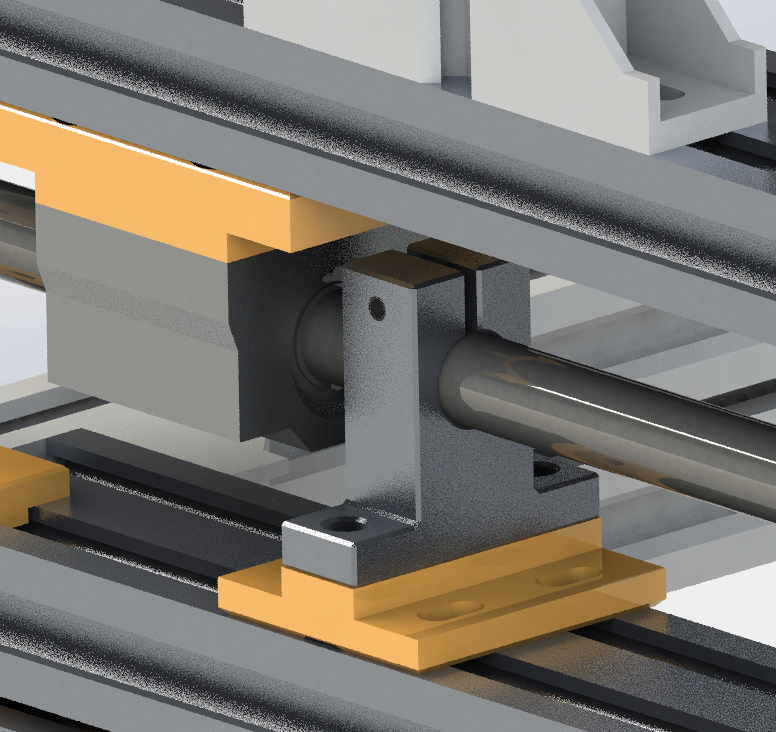
\includegraphics[width=0.4\columnwidth]{figuras/renders/suporte_sk12_com_rasgo.png}}
        \label{rasgo_suporte_sk12}
        \qquad
        \subfloat[Solução de guias lineares construída.]{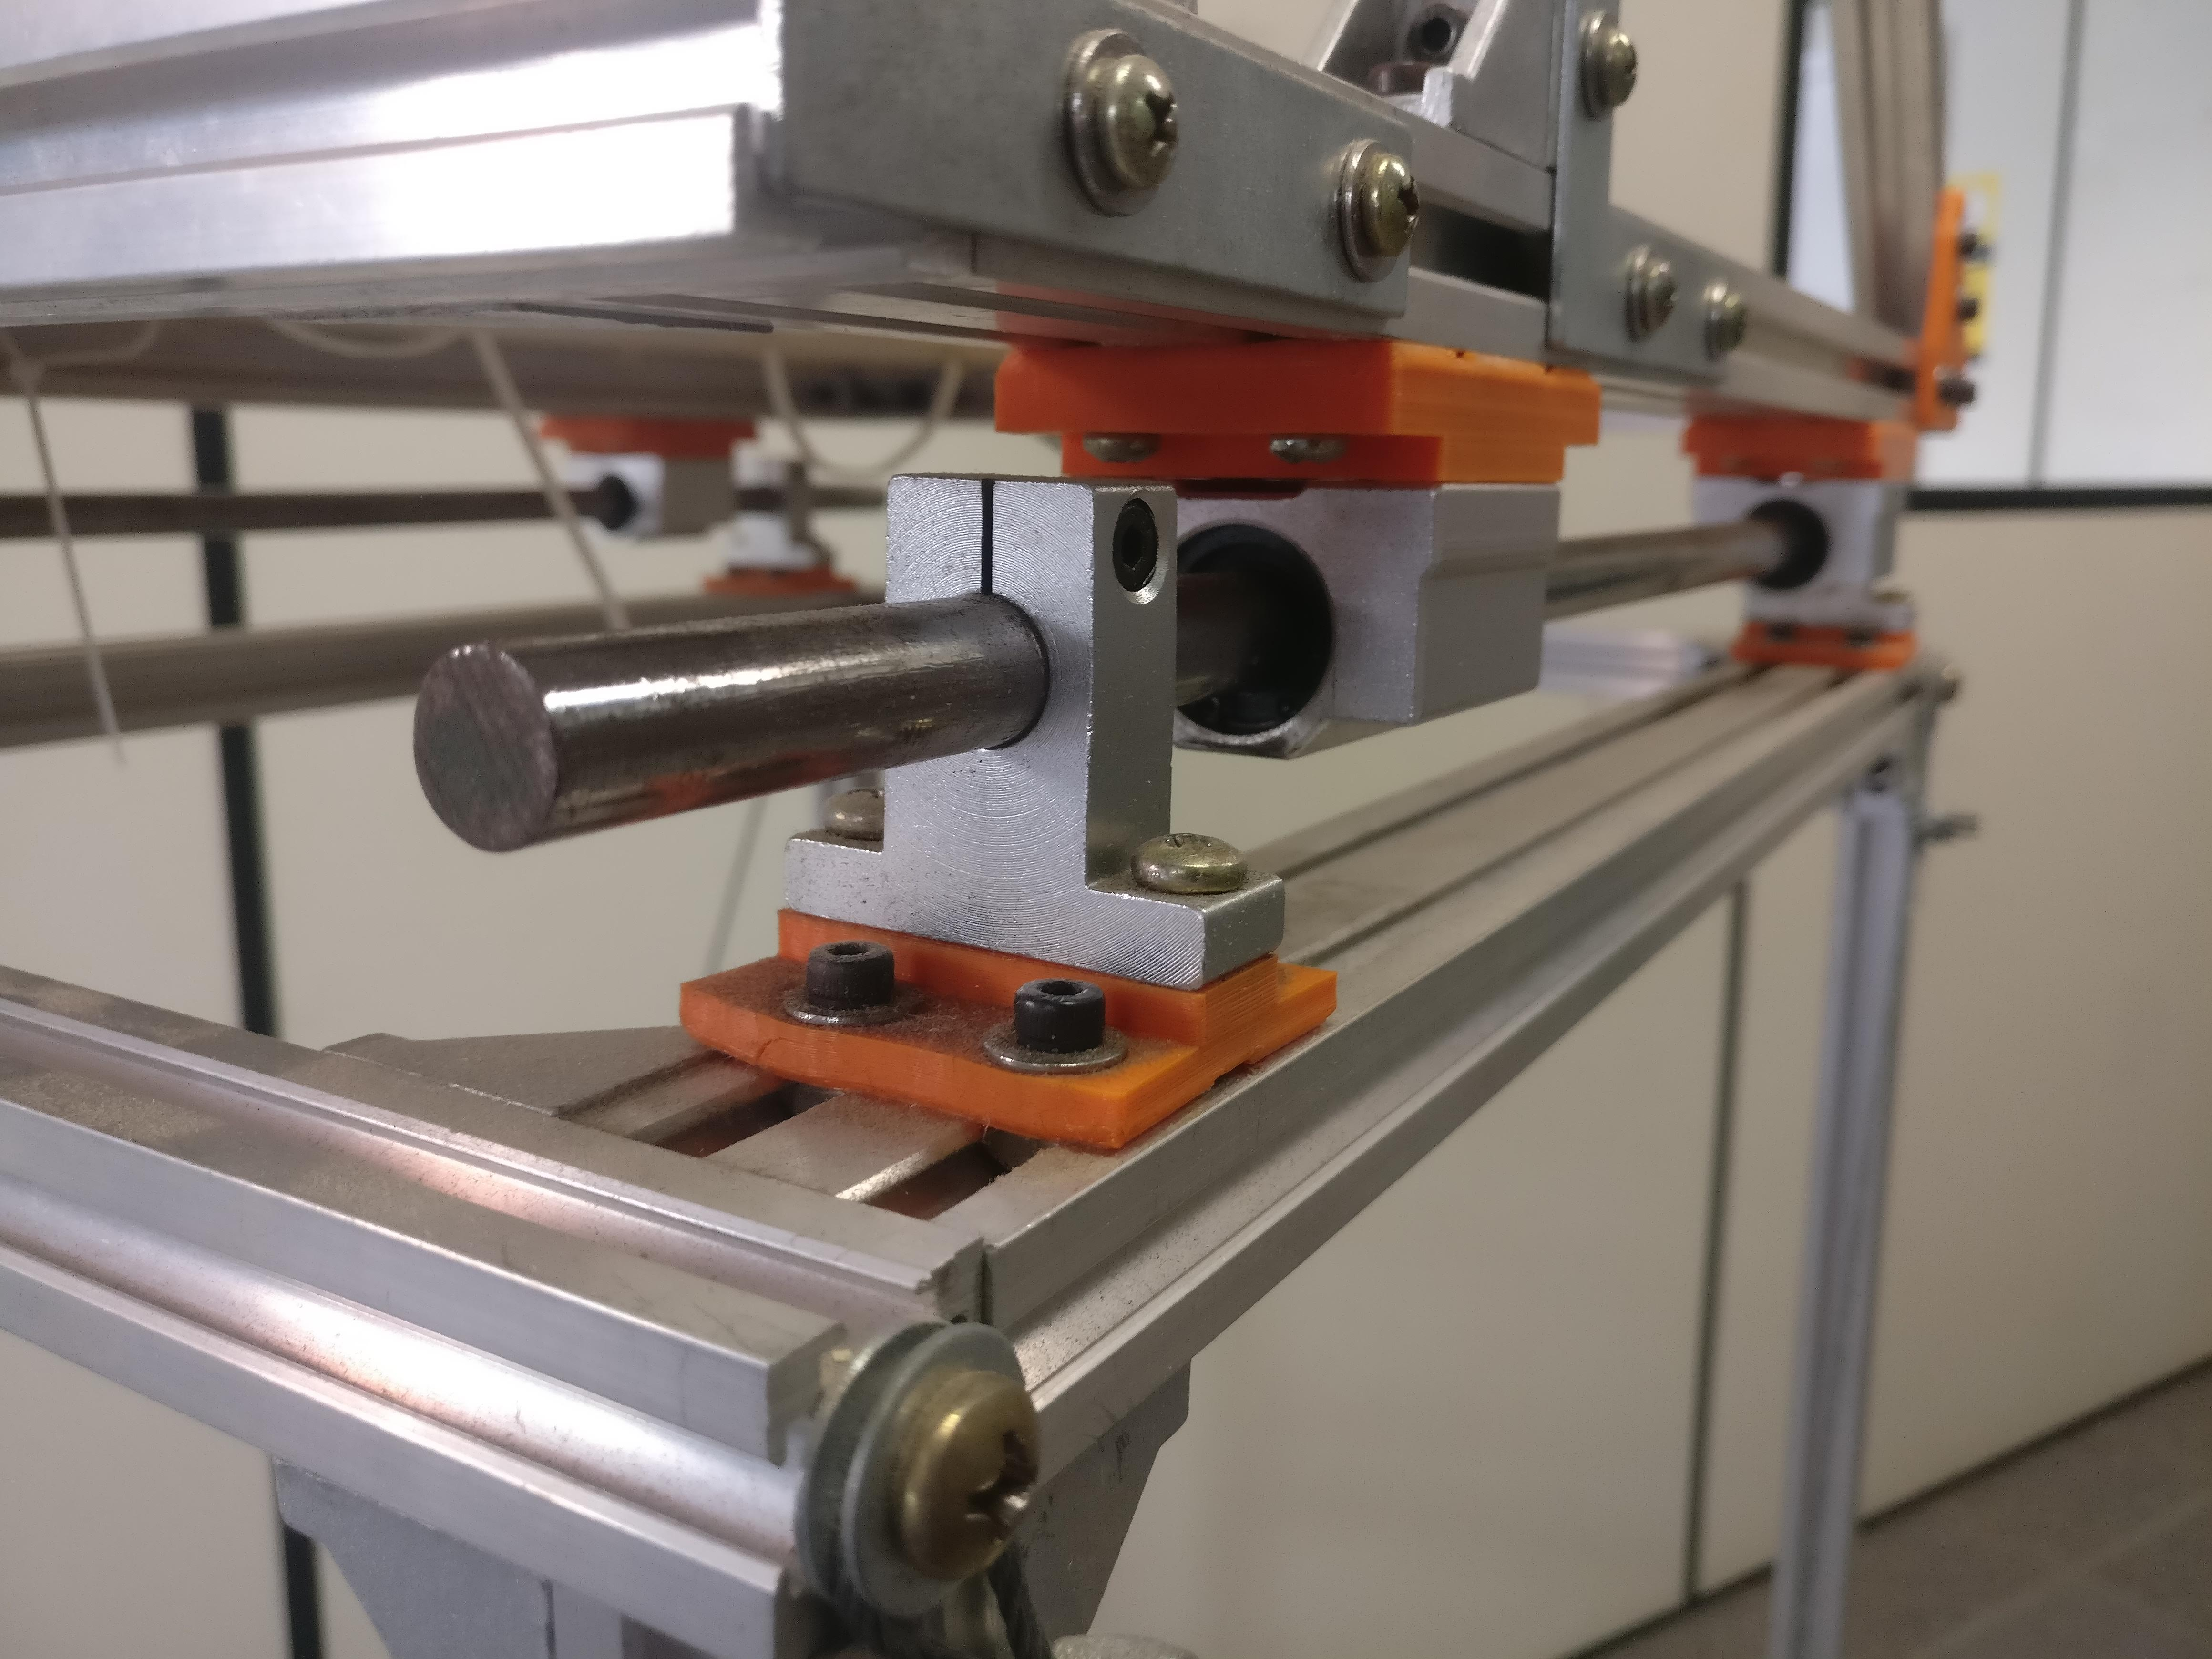
\includegraphics[width=0.4\columnwidth]{figuras/calibracao/guias_lineares.jpg}}
        \label{guias_lineares}
\end{figure}

\begin{figure}[!ht]
    \centering
    \caption{Soluções desenvolvidas para a estrutura da bancada. Fonte: O autor.}
        \subfloat[Reforço estrutural com cabos de aço.]{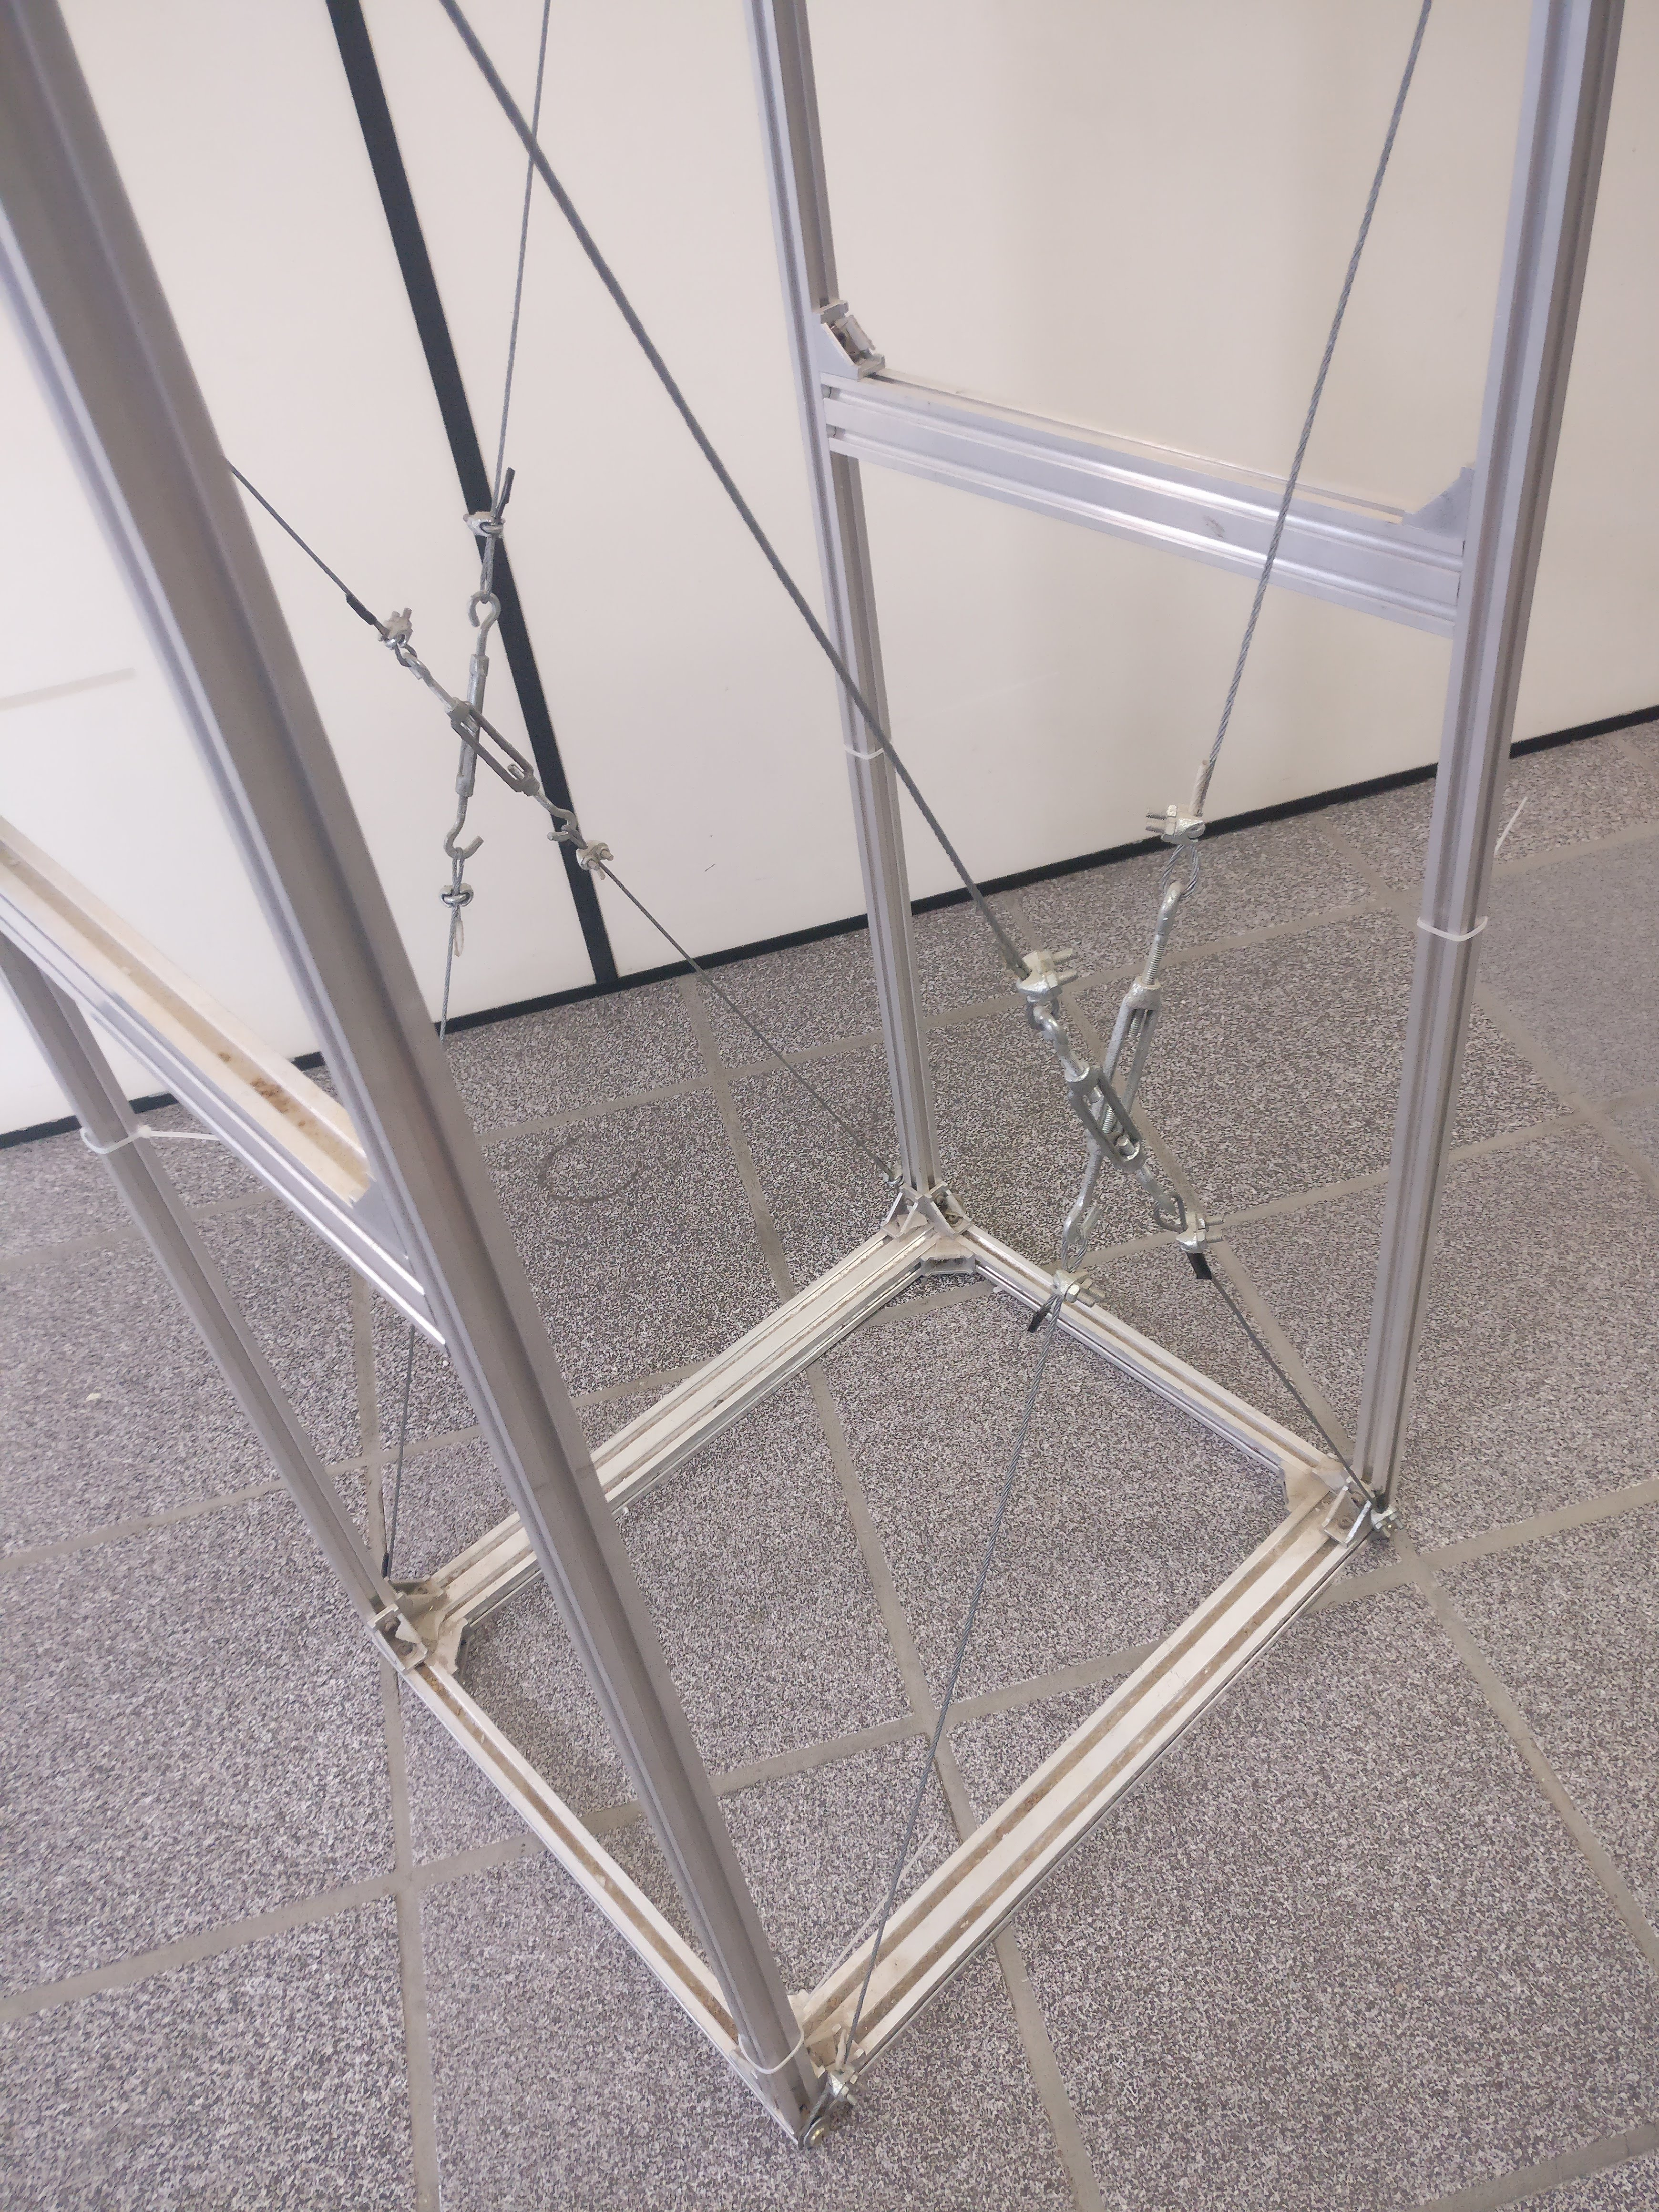
\includegraphics[width=0.4\columnwidth]{figuras/calibracao/reforco_cabos_aco.jpg}}
        \label{cabos_aco}
        \qquad
        \subfloat[Reforço estrutural utilizado nas conexões da bancada.]{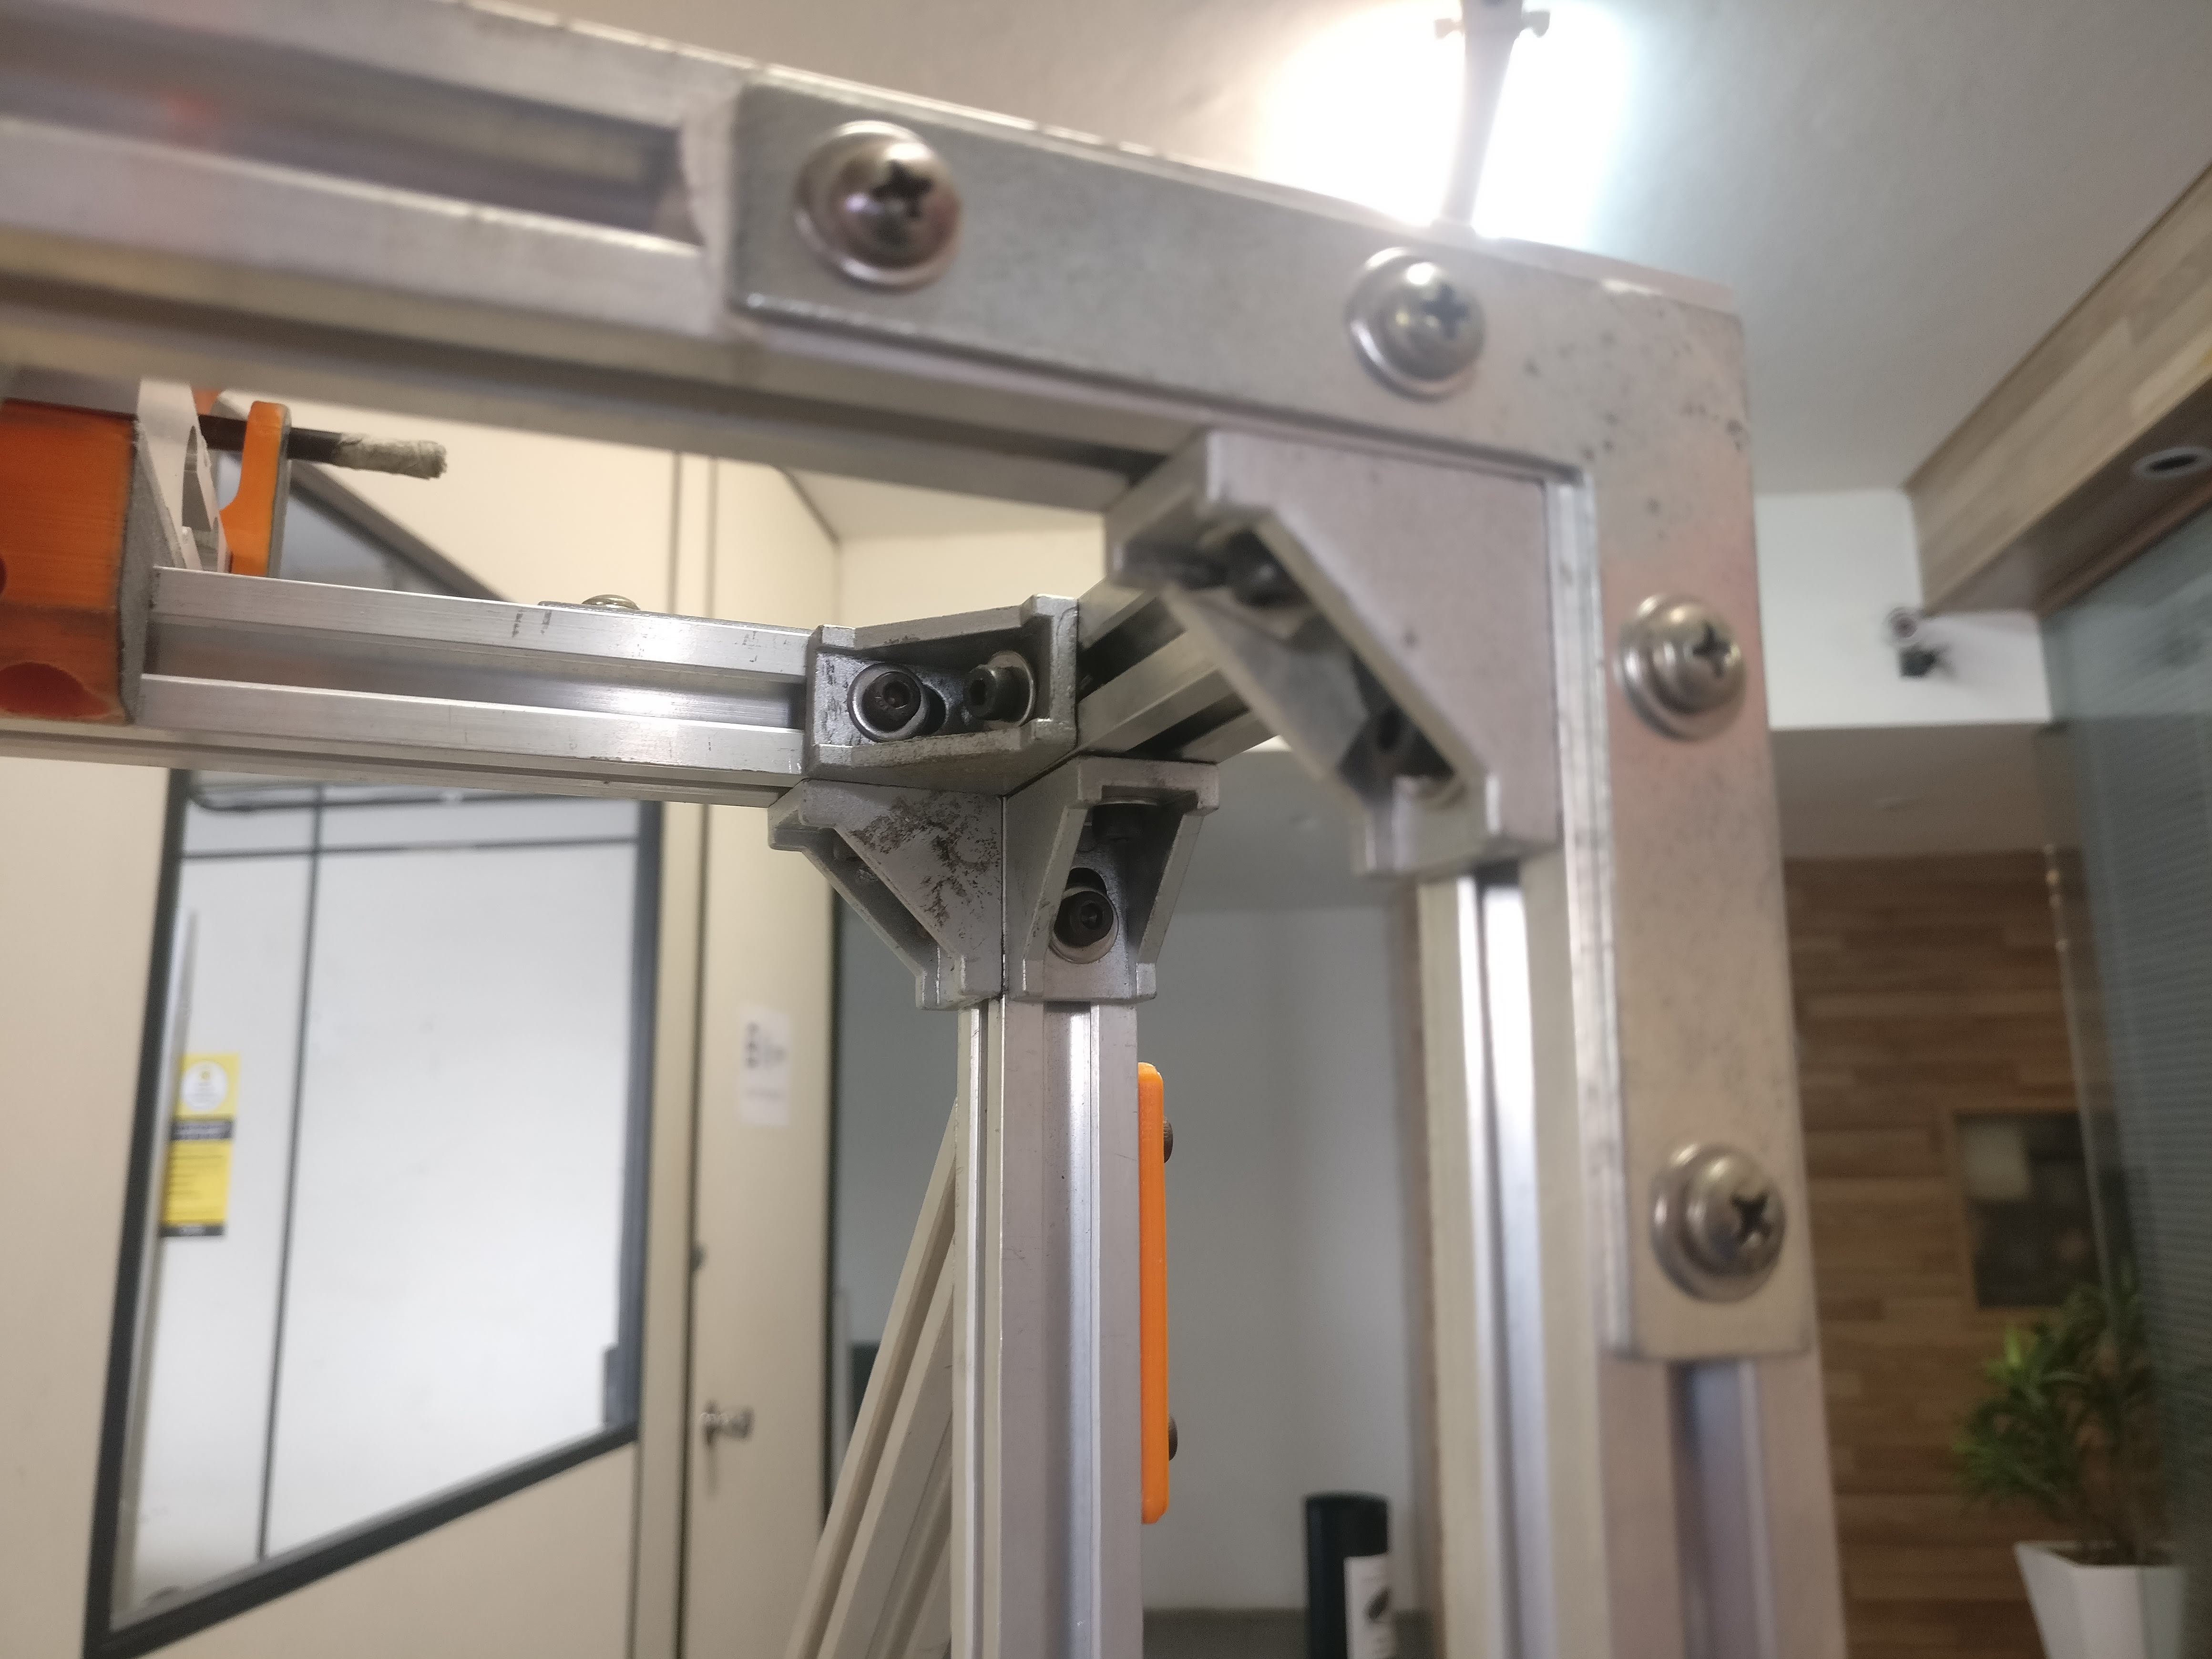
\includegraphics[width=0.4\columnwidth]{figuras/calibracao/reforco1.jpg}}
        \label{reforco_estrutural}
\end{figure}

A solução ideal para se garantir rigidez torcional da torre ao longo do eixo Z seria o treliçamento das laterais com os perfis de alumínio. Esta solução porem elevaria o custo do projeto para além do que a equipe possuía de verba disponível. A solução encontrada foi treliçar as duas laterais com cabos de aço (figura \ref{cabos_aco}).

Os furos dos quatro cantos da bancada foram rosqueados e argolas de fixação e cabos de aço foram instalados nas duas laterais, com tensionadores de modo a facilitar a instalação mesmo com pequenos desvios no comprimento dos cabos.

A primeira bancada utilizava barras roscadas como solução para o ajuste de ângulo de incidência do componente testado. Esta solução possuía três problemas principais:

\begin{itemize}
    \item Ajuste demorado, pois era necessário girar as duas barras até o ângulo desejado medindo este ângulo com o auxilio de um nível digital.
    \item Dificuldade no alinhamento da altura das duas barras, o que causava uma inclinação lateral no componente.
    \item Pouca precisão no ajuste do ângulo.
\end{itemize}

A solução encontrada foi trocar o ajuste continuo por um ajuste discreto, utilizando furos com angulação previamente projetada, como mostrado nas figuras \ref{peca_ângulo_0}a e \ref{peca_ângulo_18}b.

\begin{figure}[!ht]
    \centering
    \caption{Detalhe da peça de ajuste discreto de ângulo de incidência. Fonte: O autor.}
        \subfloat[Ajuste a 0 graus.]{\includegraphics[width=0.4\columnwidth]{figuras/renders/detalhe_ajuste_ângulo_0_graus.png}}
        \label{peca_ângulo_0}
        \qquad
        \subfloat[Ajuste a 18 graus.]{\includegraphics[width=0.4\columnwidth]{figuras/renders/detalhe_ajuste_ângulo_18_graus.png}}
        \label{peca_ângulo_18}
\end{figure}

Esta solução garante que os mesmos ângulos sempre serão utilizados nos testes, o que adiciona facilidade no processamento posterior dos dados.

Os ângulos escolhidos foram: 0, 3, 6, 9, 12, 15 e 18 graus.

O principal problema desta solução é não permitir ajustes finos no ângulo, o que a principio será um problema apenas caso se deseje descobrir o ângulo de estol de asas. Este problema porem é tido como pequeno frente aos enfrentados com a solução anterior, e pode ser contornado fabricando-se uma peça de ajuste com mais furações e/ou uma peça de ajuste continuo a ser usada especificamente no teste de estol.